\documentclass{beamer}
\let\vec\mathbf
\mode<presentation>
\usepackage{amsmath}
\usepackage{amssymb}
%\usepackage{advdate}
\usepackage{adjustbox}
%\usepackage{subcaption}
\usepackage{xparse}
\usepackage{enumitem}
\usepackage{multicol}
\usepackage{mathtools}
\usepackage{listings}
\usepackage{url}
\usepackage{gvv}
\usetheme{Boadilla}
\usecolortheme{lily}
\setbeamertemplate{footline}

{
  %\leavevmode%
  \hbox{%
  \begin{beamercolorbox}[wd=\paperwidth,ht=2.25ex,dp=1ex,right]{author in head/foot}%
    \insertframenumber{} / \inserttotalframenumber\hspace*{2ex} 
  \end{beamercolorbox}}%
  \vskip0pt%
}
\setbeamertemplate{navigation symbols}{}
\providecommand{\nCr}[2]{\,^{#1}C_{#2}} % nCr
\providecommand{\nPr}[2]{\,^{#1}P_{#2}} % nPr
\providecommand{\mbf}{\mathbf}
\providecommand{\pr}[1]{\ensuremath{\Pr\left(#1\right)}}
\providecommand{\qfunc}[1]{\ensuremath{Q\left(#1\right)}}
\providecommand{\sbrak}[1]{\ensuremath{{}\left[#1\right]}}
\providecommand{\lsbrak}[1]{\ensuremath{{}\left[#1\right.}}
\providecommand{\rsbrak}[1]{\ensuremath{{}\left.#1\right]}}
\providecommand{\brak}[1]{\ensuremath{\left(#1\right)}}
\providecommand{\lbrak}[1]{\ensuremath{\left(#1\right.}}
\providecommand{\rbrak}[1]{\ensuremath{\left.#1\right)}}
\providecommand{\cbrak}[1]{\ensuremath{\left\{#1\right\}}}
\providecommand{\lcbrak}[1]{\ensuremath{\left\{#1\right.}}
\providecommand{\rcbrak}[1]{\ensuremath{\left.#1\right\}}}
\theoremstyle{remark}

\providecommand{\res}[1]{\Res\displaylimits_{#1}} 
\providecommand{\norm}[1]{\lVert#1\rVert}
\providecommand{\mtx}[1]{\mathbf{#1}}

\providecommand{\fourier}{\overset{\mathcal{F}}{ \rightleftharpoons}}
%\providecommand{\hilbert}{\overset{\mathcal{H}}{ \rightleftharpoons}}
\providecommand{\system}{\overset{\mathcal{H}}{ \longleftrightarrow}}
\providecommand{\dec}[2]{\ensuremath{\overset{#1}{\underset{#2}{\gtrless}}}}

\title{Matrices in Geometry - 5.2.38}
\author{EE25BTECH11035  Kushal B N}
\date{Oct, 2025}

\begin{document}

\maketitle

\section{Problem Statement}
\begin{frame}
Solve the following system of equations.\\
\begin{equation*}
\frac{1}{2x}+\frac{1}{3y} = 2
\end{equation*}
\begin{equation*}
    \frac{1}{3x}+\frac{1}{2y} = \frac{13}{6}
\end{equation*}

\frametitle{Problem Statement}

\end{frame}

\section{Solution}
\begin{frame}{Solution}
Let

\begin{equation}
\vec{x} = \myvec{\frac{1}{x}\\ \frac{1}{y}}
\end{equation}

So that the given equations, after multiplying by 6 on both sides, can be represented in the matrix form as

\begin{equation}
    \myvec{3&2\\2&3}\vec{x} = \myvec{12\\13}
\end{equation}

Which can be represented as the augmented matrix
\begin{equation}
    \augvec{2}{1}{3&2&12\\2&3&13}
\end{equation}

\begin{equation}
    \augvec{2}{1}{3&2&12\\2&3&13} \xleftrightarrow{R_2 \leftarrow R_2 - \frac{2}{3}R_10} \augvec{2}{1}{3&2&12\\0&\frac{5}{3}&5}
\end{equation}

\end{frame}

\begin{frame}{Solution}
\begin{equation}
    \xleftrightarrow{R_1 \leftarrow R_1 - \frac{6}{5}R_2} \augvec{2}{1}{3&0&6\\0&\frac{5}{3}&5}
\end{equation}
So, by this, we get
\begin{equation}
    \frac{1}{y} = 3 \implies y = \frac{1}{3}
\end{equation}

\begin{equation}
    \frac{1}{x} = 2 \implies x = \frac{1}{2}
\end{equation}
\end{frame}

\section{Conclusion}
\begin{frame}{Conclusion}
$\therefore$ The solution for the given system of linear equations is $x = \frac{1}{2}$ and $y = \frac{1}{3}$.

\begin{figure}[H]
    \centering
    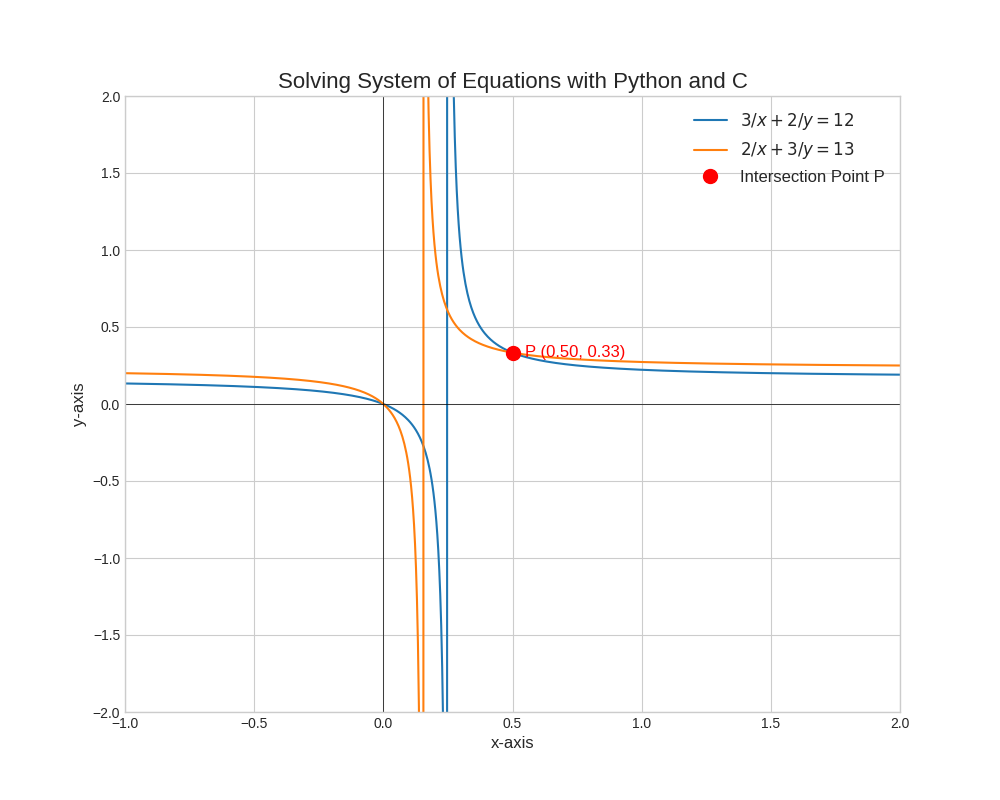
\includegraphics[width=0.73\columnwidth]{figs/1.png}
    \caption{Figure for 5.2.38}
\end{figure}
\end{frame}
\end{document}